% !TeX root = ../main.tex

\section{Caso di Studio}

\begin{frame}{Contesto Aziendale}
    % prima del contesto dire perchè è stato fatto il caso di studio: cioè l'obiettivo di dimostrare 
    % l'efficacia di devops+app multiplatform in un contesto aziendale
    \begin{columns}[onlytextwidth]
        \begin{column}{0.5\textwidth}

        \end{column}
        \begin{column}{0.5\textwidth}
             \begin{figure}[H]
                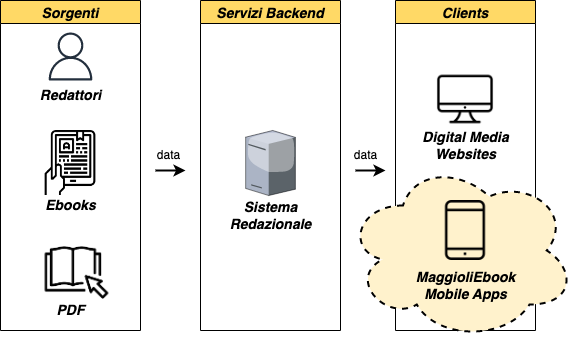
\includegraphics[width=1\textwidth]{img/contesto-aziendale.png}
            \end{figure}
        \end{column}
    \end{columns}
\end{frame}

\begin{frame}{Requisiti: Processo}
    
\end{frame}

\begin{frame}
    \begin{figure}[H]
        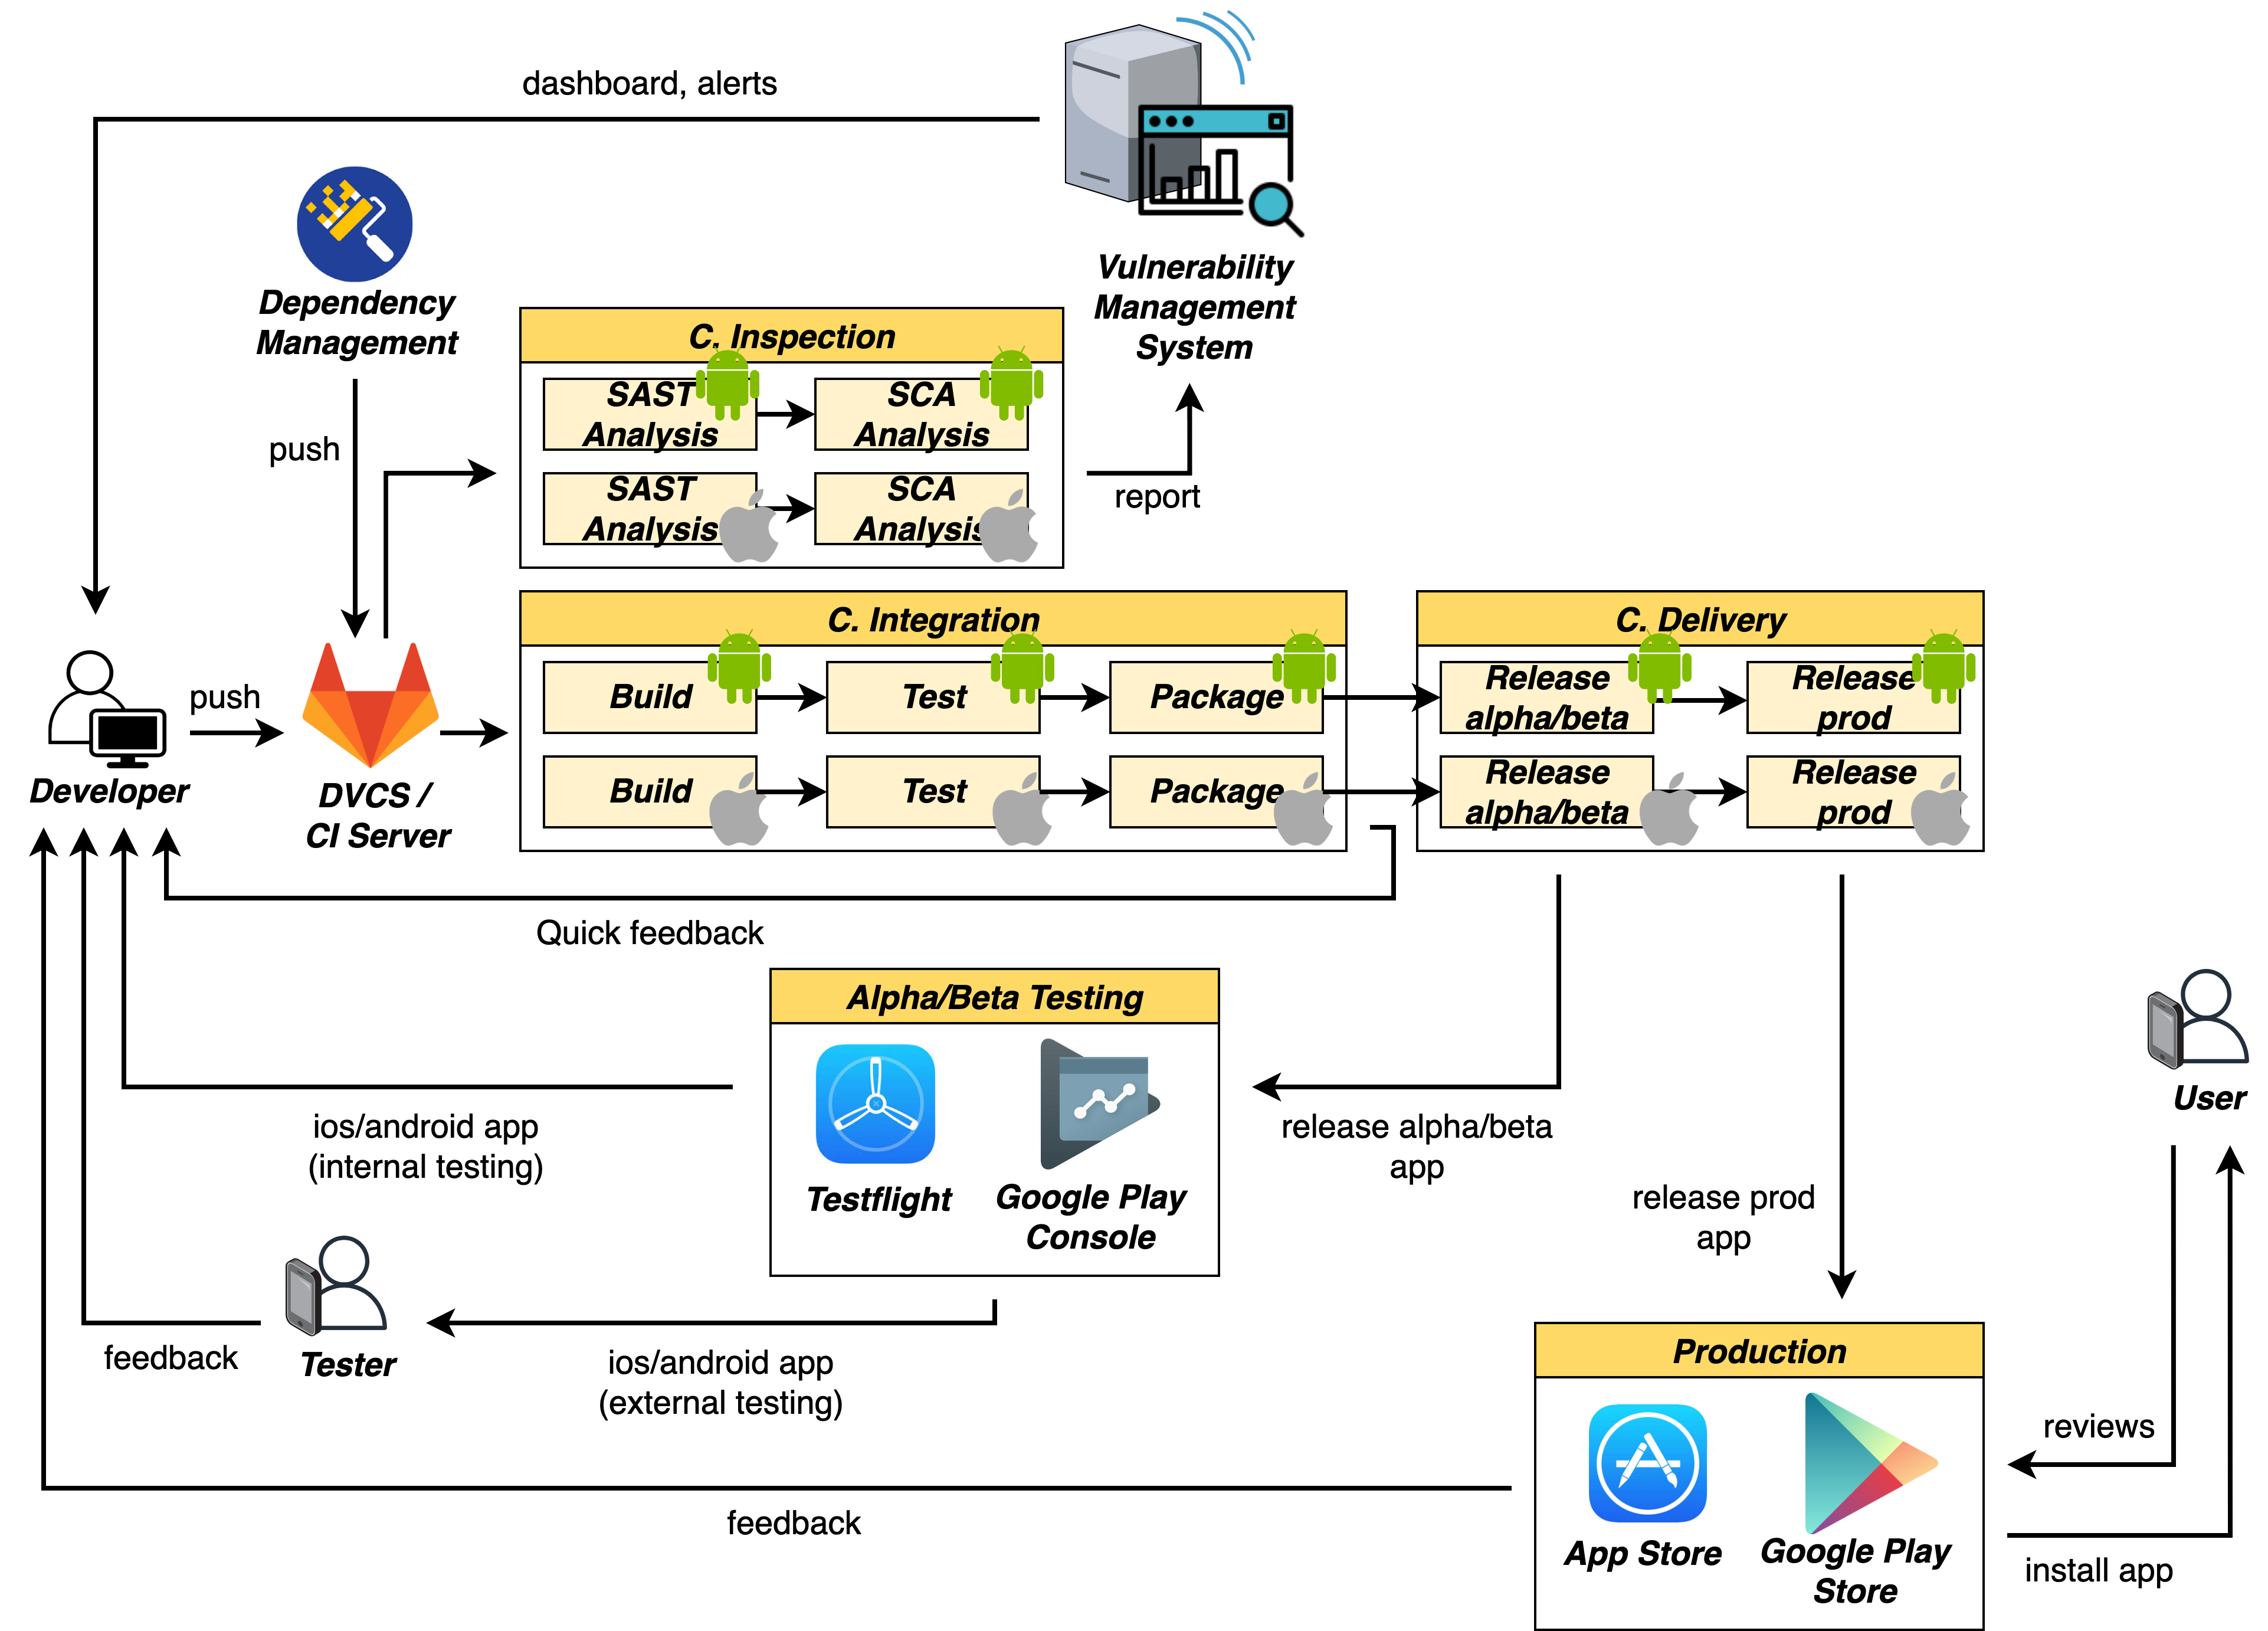
\includegraphics[width=0.82\textwidth]{img/full-cicd.png}
    \end{figure}
\end{frame}

\begin{frame}{Requisiti: Applicazione}

\end{frame}